\newcommand{\lagr}{\mathcal{L}} %likelihood
\newcommand{\LL}{\log \mathcal{L}} %likelihood
\newcommand{\sr}{\mathrm{SR}}
\newcommand{\nuis}{\theta}
\newcommand{\nuiss}{\vec{\nuis}}
\newcommand{\Pois}[2]{\mathrm{Pois}(#1 | #2)}
\newcommand{\Gaus}[3]{\mathrm{Gaus}(#1 | #2,#3)}
\newcommand{\Uniform}[3]{\mathrm{Uniform}(#1 | #2,#3)}


\subsection{The XENON1T Combined Likelihood}
%Knut
The log-likelihood used in the spin-independent analysis is a sum of extended un-binned likelihoods for the two science runs, extended un-binned likelihoods for ER calibration data, and terms expressing ancillary measurements of nuisance parameters $\nuis_m$: 
\\
Where $\sr$ runs over data-taking periods, \SRzero and \SRone, $\sigma$ is the WIMP-nucleon cross-section, and $\LL_\mathrm{sci}$,$\LL_\mathrm{cal}$ are the likelihood terms for the dark matter search data and \rnzero calibration data, respectively. Ancillary measurements  The un-binned likelihoods take the form: 

\subsection{Analysis Dimensions}
%radial choice
%benefit of less analysis space
%does FV definition go here? 
\subsection{Core Volume Segmentation}

\subsection{Safeguard}
A mismodelling term, proposed in~\cite{safeguard} is added to the ER model, consisting of a signal-like component added or subtracted to the nominal ER model: 


Since the PDF is constrained to be non-negative, the 


\subsection{Nuisance Parameters}
%Mention here: 
%BBF nuisance parameter propagation
%Radiogenics common parameter, others uncorrelated
%wall shape parameter consideration
%why signal shape was dropped
%signal rate uncertainties


\subsection{Trial Correction}
As discovery significances are computed for WIMP-masses between $6$ and $1000$ GeV, the final p-value of the experiment must reflect that multiple hypotheses were tested, and the lowest local p-value is picked as the most significant excess. The result is correlated between multiple masses, with a lower correlation between the peaked low-mass WIMP, and complete correlation between dark matter masses above $~200$ GeV, where the recoil spectrum converges. Toy Monte-Carlo data samples are generated without a dark matter signal, and discovery significances are computed for the entire mass range. The lowest local p-value is stored to compute the distribution of most significant local p-values. The global significance of the actual dataset is the percentile of the lowest p-value from the actual data of this distribution. Using local p-values rather than log-likelihood rations directly corrects for the uneven weighting that would result as different masses do not have the same null-distribution of the discovery log-likelihood ratio.


\subsection{Coverage}
The fraction of repeated experiments where the confidence interval contains the true parameter is called the coverage. Perfect coverage is equal to the confidence interval, $0.9$ in the case of XENON. As the experiment decided to report only the upper edge of the confidence interval for discovery significances $<3\sigma$, there will be over-coverage at very low signal sizes. This has a similar effect to the power constraint. Figure~\ref{fig:coverage}n shows the coverage for a $50$ GeV WIMP, with the red line representing the profile construction coverage, and blue the coverage including the $3\sigma$ threshold. The orange band, shows the $-\sigma$ to $\sigma$ sensitivity band. The result is consistent with perfect coverage (marked by the gray band, including limited statistics), with overcoverage for the $3\sigma$ threshold only under the $-1\sigma$ edge of the sensitivity band. 

\begin{figure}[tbp]
\centering
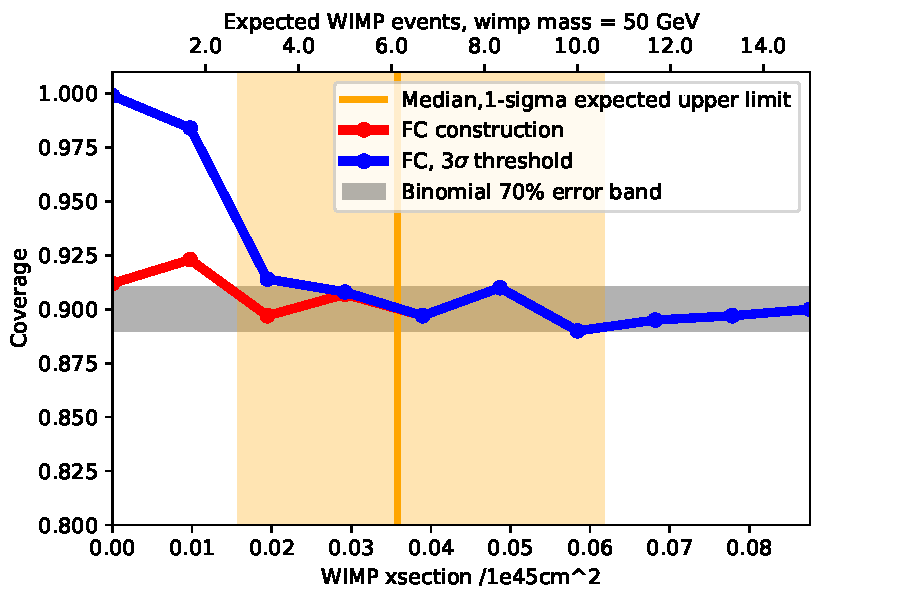
\includegraphics[width=\columnwidth]{{Plots/blueice_coverage_FCplus3sigma_wimp_mass50_livetime278.87151m}.pdf}
\caption{\label{fig:coverage} 
}
\end{figure}
